% TODO:
% - explain constraint encoding (Heule, sequential)
% - add versioning
% - add hardware specs to introduction and remove other occurrences
\section{SAT Model}
Let $X = \{x_1, x_2, ..., x_n\}$ be a set of boolean variables.
The constraints are expressed by using the following encodings: 
\begin{itemize}
    \item $AtLeastK(X), AtMostK(X)$ with a sequential encoding
    \item $ExactlyOne(X) = AtMostOne(X) \land AtLeastOne(X)$, where
    \begin{itemize}
        \item $AtLeastOne(X)=\bigvee_{i=1}^{n} x_i$
        \item $AtMostOne(X)$ with Heule Encoding
    \end{itemize}

\end{itemize}
\subsection{Decision variables}
Let $sts$ be a schedule analogous to $rb$ satisfying to the STS problem:
The satisfiability task is formalized by the following categories of propositions:

\subsubsection{Satisfiability}
% \paragraph{\text{match\_schedule}}
\begin{itemize}
    \item \textbf{match\_schedule}\\
        For each period $p \in P$ and week $w \in W$:
        $$
        match\_schedule_{p, w, m} = true
        $$
        if, and only if, the match $rb_{m, w}$ takes place in period $p$ of week $w$
    \item \textbf{match\_to\_periods}\\
        For each period $p \in P$, $t_1 \in T$ and $t_2 \in T/\{t_1\}$:
        $$
        match\_to\_periods_{t_1, t_2, p} = true
        $$
        if, and only if, $t_1$ plays against $t_2$ in period $p$.
\end{itemize}
\subsubsection{Optimization}
\begin{itemize}
    \item \textbf{flip\_slot}\\
        For each period $p \in P$ and week $w \in W$:
        $$
        flip\_slot_{p, w} = true
        $$
        if, and only if, team $sts_{p, w, 1} = t_1$ plays away
    \item \textbf{match\_to\_slots}\\
        For each $t_1 \in T$ and $t_2 \in T/\{t_1\}$:
        $$
        match\_to\_slots_{t_1, t_2} = true
        $$
        if, and only if, $t_1$ plays away and $t_2$ plays at home.
\end{itemize}

\subsection{Objective function}
Similarly to the other approaches, the objective is to minimize the absolute difference between the number of games played at home and away for each team.
Let $A_t$ and $H_t$ be the number of times the team $t \in T$ plays away and home respectively, the objective function translates into the following:
$$
k^* = \underset{k \in \mathbb{N}}{\text{argmax}} \left( \forall t \in T. (H_t \geq k \land A_t \geq k) \right)
$$
The chosen model allows to solve the optimization task using the $sts$ schedule computed in the satisfiability process. The optimization consists of a binary search of $k^*$ in the interval $[1, \lfloor\frac{N-1}{2}\rfloor]$. Since SAT doesn't directly support optimization, a new set of optimizing constraints is introduced for every instance of $k$. The constraints are defined by first binding $flip\_slots_{p, w}$ to $match\_to\_slots_{p, w}$:
$$
    \forall p \in P, w \in W.(flip\_slot_{p, w} \leftrightarrow match\_to\_slots_{sts_{p, w, 0}, sts_{p, w, 1}})
$$
and then enforcing, for any $k$, that $t_1$ plays at least $k$ times away and at $k$ times at home:
$$
\begin{aligned}
    &\forall p \in P,\ \forall t_1 \in T.( \text{AtLeastK}(match\_to\_slots_{t_1,t_2} \mid t_2 \in T \setminus \{t_1\})\\
    &\left. \land\ 
    \text{AtLeastK}(\lnot match\_to\_slots_{t_1,t_2} \mid t_2 \in T \setminus \{t_1\}) \right)
\end{aligned}
$$

\subsection{Constraints}
\subsubsection{Each match is assigned to a unique period each week}
For each week $w$ we ensure that every match is assigned to one period $p$
$$
    \forall p \in P, w \in W.(ExactlyOne(match\_schedule_{p, w, m} | m \in M))
$$
and every period is assigned to one match
$$
    \forall m \in M, w \in W.(ExactlyOne(match\_schedule_{p, w, m} | p \in P))
$$
\subsubsection{Every team plays at most twice in the same period}
First we bind $match\_schedule_{p, w, m}$ to $match\_to\_periods_{t_1, t_2, p}$:
% The constraint cannot be expressed using directly $match\_schedule_{p, w, m}$, due to structural limitations of the encoding. 
% Instead, $match\_to\_periods_{t_1, t_2, p}$ is used: given a week $w$, the match $rb_{m,w}$ is scheduled in period $p$ if, and only if, the match $(rb_{m, w, 1}, rb_{m, w, 2}) = (t_1, t_2)$ takes place in period $p$. Therefore, by definition: 
$$
    \forall p \in P, w \in W, m \in P.(match\_schedule_{p, w, m} \leftrightarrow match\_to\_periods_{rb_{m, w, 0}, rb_{m, w, 1}, p})
$$
and then enforcing that $t_1$ plays at most 2 times in period $p$:
$$
    \forall p \in P, t_1 \in T. AtMost2(match\_to\_periods_{t_1, t_2, p} | t_2 \in T/\{t_1\})
$$
\subsection{Validation}
\subsubsection{Experimental design}
The model was written in Python by making use of the Z3 4.15.1.0 and the CVC5 1.3.0 libraries, which offers CaDiCaL and MiniSat as the underlying SAT solvers.
The objective values found within the 300 second time limit, are presented in Table~\ref{table:sat-results}. 
\subsubsection{Experimental results}
All solvers either find the optimal solution or no solution at all. Overall Z3 was the fastest and was able to solve the problems with higher $N$, reaching $N=20$. On the other hand CaDiCaL was the worst, failing at $N=12$, while MiniSat stopped at $N=14$

\begin{table}[ht]
\centering
\begin{tabular}{|c|c|c|c|}
\toprule
\textbf{n} & \textbf{Z3} & \textbf{MiniSat} & \textbf{CaDiCaL} \\
\midrule
\textbf{6}  & \textbf{2}   & \textbf{2}   & \textbf{2}   \\
\textbf{8}  & \textbf{3}   & \textbf{3}   & \textbf{3}   \\
\textbf{10} & \textbf{4}   & \textbf{4}   & \textbf{4}   \\
\textbf{12} & \textbf{5}   & \textbf{5}   & N/A         \\
\textbf{14} & \textbf{6}   & N/A         & N/A         \\
\textbf{16} & \textbf{7}   & N/A         & N/A         \\
\textbf{18} & \textbf{8}   & N/A         & N/A         \\
\textbf{20} & \textbf{9}   & N/A         & N/A         \\
\textbf{22} & N/A          & N/A         & N/A         \\
\bottomrule
\end{tabular}
\caption{SAT optimization solver results}
\label{table:sat-results}
\end{table}


% \begin{figure}[H]
%     \centering
%     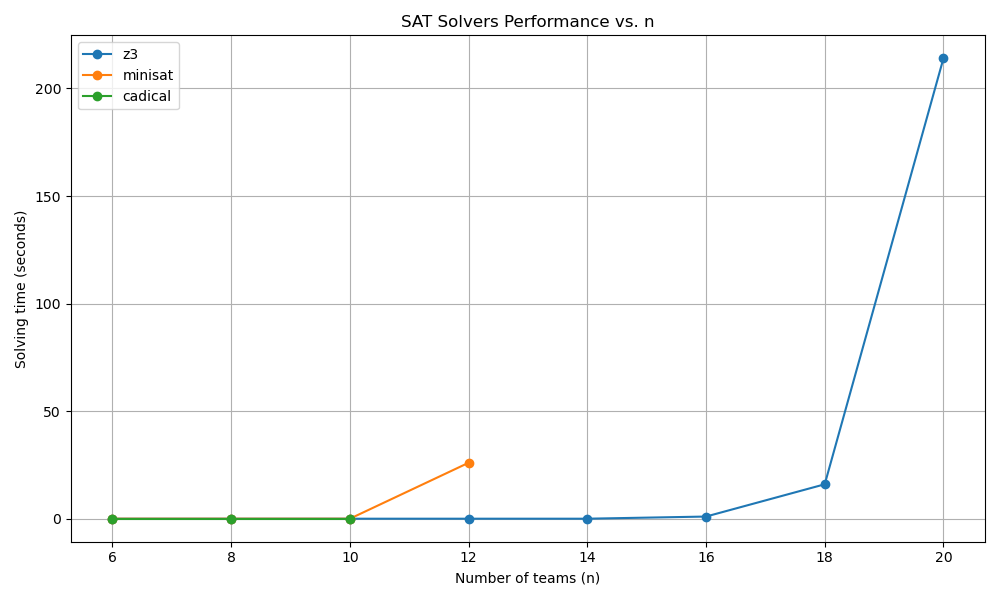
\includegraphics[width=0.8\linewidth]{img/SAT-result.png}
%     \caption{SAT optimization}
%     \label{fig:SAT-result}
% \end{figure}
